\documentclass[10pt,a4paper,oneside]{beamer}
\usepackage[utf8]{inputenc}
\usepackage{amsmath}
\usepackage{amsfonts}
\usepackage{amssymb}
\usepackage{graphicx}
\usepackage{breqn}
\usepackage{tikz} % system block diagram
\usepackage{textcomp}
\usetikzlibrary{shapes,arrows} % system block diagram
\usepackage{booktabs}
\usepackage[framed,numbered,autolinebreaks,useliterate]{mcode} % matlab code block
\author{Yangang Cao}
\newcommand{\degree}{^\circ}
\tikzset{
	delay/.style    = {draw, thick, rectangle, minimum height = 3em,
		minimum width = 3em},
	sum/.style      = {draw, circle, node distance = 2cm}, 
	prod/.style     = {draw, circle, node distance = 2cm},
	input/.style    = {coordinate}, % Input
	output/.style  = {coordinate} % Output
}
% Defining string as labels of certain blocks.
\newcommand{\product}{$\displaystyle \times$}
\newcommand{\delay}{\large$z^{-1}$}
%\documentclass[aspectratio=169]{beamer}
\usepackage[english]{babel}

% 加导航条
%\useoutertheme[width=3\baselineskip,right]{sidebar}
% 目录标数字
\setbeamertemplate{section in toc}[sections numbered] 
% 无序列表用实心点
\setbeamertemplate{itemize item}{$\bullet$}
% 设置每页标题格式
\setbeamertemplate{frametitle}
{\vspace{-0.5cm}
	\insertframetitle
	\vspace{-0.5cm}}
% 去掉下面没用的导航条
\setbeamertemplate{navigation symbols}{}
% 设置页脚格式
\makeatother
\setbeamertemplate{footline}
{
	\leavevmode%
	\hbox{%
		\begin{beamercolorbox}[wd=.4\paperwidth,ht=2.25ex,dp=1ex,center]{author in head/foot}%
			\usebeamerfont{author in head/foot}\insertshortauthor
		\end{beamercolorbox}
		
		\begin{beamercolorbox}[wd=.6\paperwidth,ht=2.25ex,dp=1ex,center]{title in head/foot}%
			\usebeamerfont{title in head/foot}\insertshorttitle\hspace*{13em}
			\insertframenumber{} / \inserttotalframenumber\hspace*{0ex}
	\end{beamercolorbox}}
	
	\vskip0pt%
}
\makeatletter


% 定义颜色
%\definecolor{alizarin}{rgb}{0.82, 0.1, 0.26} % 红色
%\definecolor{DarkFern}{HTML}{407428} % 绿色
%\colorlet{main}{DarkFern!100!white} % 第一种设置方法
%\colorlet{main}{red!70!black} % 第二种设置方法
\definecolor{bistre}{rgb}{0.24, 0.17, 0.12} % 黑色
\definecolor{mygrey}{rgb}{0.52, 0.52, 0.51} % 灰色
\colorlet{main}{green!50!black}
\colorlet{text}{bistre!100!white}

% 不同元素指定不同颜色,fg是本身颜色,bg是背景颜色,!num!改变数值提供渐变色
\setbeamercolor{title}{fg=text}
\setbeamercolor{frametitle}{fg=main}
\setbeamercolor{section in toc}{fg=text}
\setbeamercolor{normal text}{fg=text}
\setbeamercolor{block title}{fg=main,bg=mygrey!14!white}
\setbeamercolor{block body}{fg=black,bg=mygrey!10!white}
\setbeamercolor{qed symbol}{fg=main} % 证明结束后的框颜色
\setbeamercolor{math text}{fg=black}
% 设置页脚对应位置颜色
\setbeamercolor{author in head/foot}{fg=black, bg=mygrey!5!white}
\setbeamercolor{title in head/foot}{fg=black, bg=mygrey!5!white}
\setbeamercolor{structure}{fg=main, bg=mygrey!10!white} % 设置sidebar颜色

% 左右页间距的排版
\def\swidth{1cm}
\setbeamersize{sidebar width right=\swidth}
\setbeamersize{sidebar width left=\swidth}
\setbeamerfont{title in sidebar}{size=\scriptsize}
\setbeamerfont{section in sidebar}{size=\tiny}


%-------------------正文-------------------------%

\author{Yangang Cao}
\title{Second-Order Bandpass/Bandreject Filter Design}
\date{February 15, 2019}

\begin{document}
	
	\frame[plain]{\titlepage}
	

\begin{frame}
\frametitle{Definition of Bandpass/Bandreject Filter}
\vspace{1.5cm}
 Definition of Bandpass/Bandreject filter:
\vspace{0.3cm}
\begin{itemize}
	\item {\bfseries Bandpass (BP)} filters select frenquencies between a lower cut-off frenquency $f_{cl}$ and a higher cut-off frenquency $f_{ch}$. Frenquencies below $f_{cl}$ and frenquencies higher than $f_{ch}$ are attenuated.
	\item {\bfseries Bandreject (BR)} filters attenuate frenquencies between a lower cut-off frenquency $f_{cl}$ and a higher cut-off frenquency $f_{ch}$. Frenquencies below $f_{cl}$ and frenquencies higher than $f_{ch}$ are passed.
\end{itemize}
\end{frame}

\begin{frame}
Second-order bandpass and bandreject filters can be described by the following transfer function
\[
H(z) = \frac{1}{2}[1 \mp A(z)]\quad(BP/BR-/+)
\]
\[
A(z) = \frac{-c + d(1-c)z^{-1} + z^{-2}}{1 + d(1-c)z^{-1} - cz^{-2}}
\]
\[
c = \frac{\tan(\pi f_b/f_S) - 1}{\tan(\pi f_b/f_S) + 1}
\]
\[
d = -\cos(2\pi f_c/f_S),
\]
where a tunable second-order allpass $A(z)$ with tuning parameters $c$ and $d$ is used. The minus sign (-) denotes the bandpass operation and the plus sign (+) the bandreject operation.
\end{frame}

\begin{frame}
Block diagram of second-order bandpass/bandreject filter:
\begin{center}
	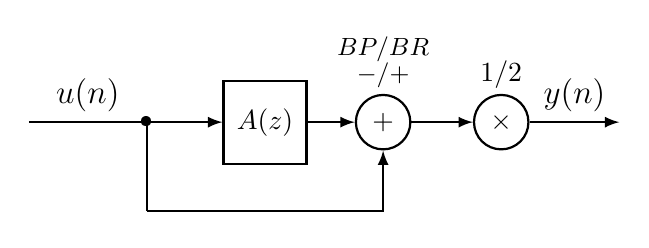
\begin{tikzpicture}[auto, thick, node distance=0.6cm, >=latex, scale = 0.75]
	\draw
	node at (2,0)[delay] (d1) {$A(z)$}
	node at (4,0)[sum] (s1) {$+$} 
	node[above of = s1]{\small$-/+$} node[above of=s1,above=1]{\small{$BP/BR$}}
	node at (6,0) [prod] (p1) {\product} node[above of = p1]{$1/2$};
	
	\draw[-](-2,0) -- node {\large$u(n)$}(0,0);
	\draw[->](0,0) -- node {} (d1);
	\draw[->](d1) -- node {} (s1);
	\draw[->](s1) -- node {} (p1);
	\draw[->](p1) -- node {\large$y(n)$} (8,0);
	\draw[-](0,0) -- node {} (0,-1.5);
	\draw[->](0,-1.5) -| node {} (s1);
	
	\draw
	node at (0,0) {\textbullet};
	\end{tikzpicture}
\end{center}
\end{frame}
\begin{frame}
The difference equations of second-order bandpass filter are
\[
x(n) = u(n) - d(1-c)x(n-1) + cx(n-2)
\]
\[
y(n) = \frac{1+c}{2}x(n) - \frac{1+c}{2}x(n-2),
\]
and corresponding state and output equations are
\[
\begin{bmatrix}x(n)\\x(n-1)\end{bmatrix} = \begin{bmatrix}
-d(1-c)&c\\
1&0
\end{bmatrix}
\begin{bmatrix}x(n-1)\\x(n-2)\end{bmatrix} + \begin{bmatrix}1\\0\end{bmatrix}
u(n)\]
\[
y(n) = \begin{bmatrix}\frac{d(c^2-1)}{2}&\frac{c^2-1}{2}\end{bmatrix}
\begin{bmatrix}x(n-1)\\x(n-2)\end{bmatrix} + \frac{1+c}{2}u(n).
\]
\end{frame}
\begin{frame}[fragile]
Matlab code:
\begin{lstlisting}
function y = apbandpassunit(audio, para)
% Applies a bandpass filter to the input signal.
% para(1) is the normalized center frequency in (0,1), i.e. 2*fc/fs.
% para(2) is the normalized bandwidth in (0,1) i.e. 2*fb/fs.
c = (tan(pi*para(2)/2)-1) / (tan(pi*para(2)/2)+1);
d = -cos(pi*para(1));
x = [0; 0];
x_1 = 0;
A = [-d*(1-c), c; 1, 0];
B = [1; 0];
C = [d*(c^2-1)/2, (c^2-1)/2];
D = (1+c)/2;
for n=1:length(audio)
    x_1 = A * x + B * audio(n);
    y(n) = C * x + D * audio(n);
    x = x_1;
end
\end{lstlisting}
\end{frame}
\begin{frame}
The difference equations of second-order bandreject filter are
\[
x(n) = u(n) - d(1-c)x(n-1) + cx(n-2)
\]
\[
y(n) = \frac{1-c}{2}x(n) + d(1-c)x(n-1) + \frac{1-c}{2}x(n-2),
\]
and corresponding state and output equations are
\[
\begin{bmatrix}x(n)\\x(n-1)\end{bmatrix} = \begin{bmatrix}
-d(1-c)&c\\
1&0
\end{bmatrix}
\begin{bmatrix}x(n-1)\\x(n-2)\end{bmatrix} + \begin{bmatrix}1\\0\end{bmatrix}
u(n)\]
\[
y(n) = \begin{bmatrix}\frac{d(1-c^2)}{2}&\frac{1-c^2}{2}\end{bmatrix}
\begin{bmatrix}x(n-1)\\x(n-2)\end{bmatrix} + \frac{1-c}{2}u(n).
\]
\end{frame}
\begin{frame}[fragile]
Matlab code:
\begin{lstlisting}
function y = apbandrejectunit(audio, para)
% Applies a bandreject filter to the input signal.
% para(1) is the normalized center frequency in (0,1), i.e. 2*fc/fs.
% para(2) is the normalized bandwidth in (0,1) i.e. 2*fb/fs.
c = (tan(pi*para(2)/2)-1) / (tan(pi*para(2)/2)+1);
d = -cos(pi*para(1));
x = [0; 0];
x_1 = 0;
A = [-d*(1-c), c; 1, 0];
B = [1; 0];
C = [d*(1-c^2)/2, (1-c^2)/2];
D = (1-c)/2;
for n=1:length(audio)
    x_1 = A * x + B * audio(n);
    y(n) = C * x + D * audio(n);
    x = x_1;
end
\end{lstlisting}
\end{frame}
\end{document}